%-----------------------------------------------------------------------------------------------
% 2020-NaaktgeborenC-PolyProc.tex - by C. Naaktgeboren
% License: CC-BY-NC-ND 4.0 - https://creativecommons.org/licenses/by-nc-nd/4.0/
%-----------------------------------------------------------------------------------------------
\documentclass[10pt,a4paper]{article}
%-----------------------------------------------------------------------------------------------
\usepackage[top=25mm,bottom=25mm,left=25mm,right=25mm]{geometry}
\usepackage{authblk}
\usepackage{pslatex}
\usepackage{graphicx}
\usepackage[squaren,cdot]{SIunits}
\usepackage{multicol}
\usepackage{float}
\usepackage{amsthm}
%-----------------------------------------------------------------------------------------------
\setlength{\columnsep}{8mm}
\setlength{\columnseprule}{0.4pt}
%-----------------------------------------------------------------------------------------------
\newtheorem{theorem}{Theorem}
\newtheorem{definition}{Definition}
\newtheorem{example}{Example}
%-----------------------------------------------------------------------------------------------
\makeatletter
\immediate\write18{datelog > \jobname.info} % site script: $(date -u '+%Y-%m-%d %Hh%Mm%Ss UTC')
\makeatother
%-----------------------------------------------------------------------------------------------
\renewcommand\Affilfont{\itshape\small}
%-----------------------------------------------------------------------------------------------
\title{%
    On Exact and Local Polytropic Processes -- Requisites, Etymology, and Modeling \\[1.0ex]
    {\normalsize\sc A Preprint}
}
\author[1]{C.~Naaktgeboren}
\affil[1]{%
    Universidade Tecnológica Federal do Paraná -- UTFPR, Câmpus Guarapuava.\par
    Grupo de Pesquisa em Ciências Térmicas.
}
\date{{\scriptsize\tt%
    \includegraphics[height=6.0mm]{cc/by-nc-nd.pdf}\\
    Compiled on \input{\jobname.info}
}}
%-----------------------------------------------------------------------------------------------
\begin{document}
%-----------------------------------------------------------------------------------------------

\maketitle

\begin{abstract}
    Work in progress.
    Here goes the abstract...
\end{abstract}
\vspace{0.5ex}

%-----------------------------------------------------------------------------------------------
{
    \small\noindent\textbf{Keywords:}~Thermodynamics,  Polytropic  Processes,  Logical  Process,
    Etymology, Modeling.
} \vspace{1.5ex}

%-----------------------------------------------------------------------------------------------
{
    \small\noindent\textbf{Remarks:}~~%
    $\bullet$~Defines \emph{logical thermodynamic process}
    $\bullet$~Defines \emph{exact polytropic process}
    $\bullet$~Brings new definition for \emph{local polytropic process}
    $\bullet$~Defines theoretical \emph{requisites} for exact polytropic process.
} \vspace{1.5ex}

%-----------------------------------------------------------------------------------------------
\begin{multicols*}{2}

%-----------------------------------------------------------------------------------------------
\section{Introduction}

    Many equilibrium engineering thermodynamics processes  are  taken  to  follow  a  polytropic
    relationship of constant $Pv^n$, in which $P$ is the system pressure, in  \kilo\pascal,  $v$
    is the system specific volume, in $\meter\cubed\!\per\kilogram$, and $n$ is a  dimensionless
    polytropic exponent~\cite{2013-CengelYA+BolesMA-AMGH}; which means, for a ``1--2''  process,
    with end states labeled as ``1'' and ``2'', the relation $P_1v_1^n = P_2v_2^n$ holds true.

    Some maintream thermodynamics textbooks introduce polytropic processes  in  the  context  of
    closed system boundary work, as a  $P:P(v)$  relationship  to  plug  in  the  boundary  work
    integral,   which    contains    a    $P\,dv$    integrand~\cite{2013-CengelYA+BolesMA-AMGH,
    2002-MoranMJ+ShapiroHN-LTC, 1985-WylenG-Wiley}. In such texts, the  polytropic  relationship
    is frequently said to find support in measurents, while no specific  theoretical  derivation
    is presented at the point of introduction.

    On  the  other  hand,  other  texts~\cite{1986-JonesJB+HawkinsGA-Wiley,   2006-BejanA-Wiley,
    2015-KroosKA+PotterMC-Cengage} include derivations that lead to a polytropic process, or  at
    least to an isentropic version of it, in which the exponent $n$ has a fixed value.

    Moreover, Bejan~\cite[p.~175]{2006-BejanA-Wiley} indicates that a constant  $Pv^n$  relation
    only holds \emph{locally} if the process is such that $n$ is a function of either $P$,  $v$,
    or both.

    A paper due to Christians~\cite{2012-ChristiansJ-IntJMechEngEduc} discusses the topic from a
    perspective  of  teaching  polytropic  processes  themselves,  placing   emphasis   on   the
    \emph{heat-to-work transfer ratio}---named by that author as ``energy transfer ratio''---and
    how its constancy not only yields, but constitutes a  pre-requisite  for  a  process  to  be
    polytropic, besides, naturally, the constancy of the caloric properties of the working  pure
    substance.

    This work develops the concepts of \emph{exact} and \emph{local} polytropic  processes,  and
    presents theory-derived \emph{requisites} for a process to be exactly polytropic.  Moreover,
    an  \emph{etymological}  discussion  is  presented  in  connection  to  the  usefulness   of
    \emph{local} polytropic processes for  generalized  equilibrium  engineering  thermodynamics
    process \emph{modeling}.

%-----------------------------------------------------------------------------------------------
\section{Exact and Local Polytropic Processes}

    In equilibrium engineering thermodynamics, a \emph{process}---more properly  a  quasi-static
    or quasi-equilibrium process---is defined in terms of changes  from  a  certain  equilibrium
    state of a system to  another~\cite{2013-CengelYA+BolesMA-AMGH},  with  process  \emph{path}
    being the (infinite) sequence of (quasi-)equilibrium states visited by the system during the
    process. A process can be referred to by its path, with implicit or explicit end states.

    It is worth noting that no constraints are stated for the end  states  of  a  process.  This
    allows for the needed flexibility in describing the variety of  transformations  on  systems
    and control volumes possible in engineering thermodynamics.

    This lack of end state constraints in the definition of a process  allows  processes  to  be
    splitted into multiple sub-processes that still fit the definition of a process, as well as
    merged together into super-processes that also fit the definition of a process.

    In order  to  make  the  intended  distinction  between  proposed  ``exact''  and  ``local''
    polytropic processes, additional constraints need to be made  to  process  end  states.  The
    following defines a \emph{logical} (thermodynamic) \emph{process}, which is a  process  with
    constrained end states:

    \begin{definition}[logical process]\label{def:logical.proc}
        Define logical process as one in which its stated defining conditions,  that  determines
        all of the allowed interactions or property  relations  for  the  underlying  system  or
        control volume, apply uniformly from, but not earlier than, its initial state until, but
        not later than, its end state.
    \end{definition}

    Therefore,   for   a   simple   compressible   system---admitting   only   work   and   heat
    interactions---either stated heat and work interactions, or system property  specifications,
    or combinations of the two, define possible logical processes.

    \begin{example}\label{ex:ideal.Diesel}
        The   well-known   air-standard   ideal   Diesel    power    cycle,    illustrated    on
        Figure~\ref{fig:cycle.Diesel},  with  ``intake''  state  (of  lowest   temperature   and
        pressure) labeled as ``1'',  can  be  divided  in  different  ways  using  only  logical
        processes.  One  such  division  is:  (i)~``isentropic  compression'',   (ii)~``isobaric
        heating'',  (iii)~``isentropic  expansion'',  and  (iv)~``isochoric   cooling'',   which
        correspond to the ``1--2'', ``2--3'', ``3--4'', and ``4--1'',  respectively,  i.e.,  the
        canonical  processes  for  this  cycle.  Other  possibilities  include:  (a)~``any  work
        temperature increase'', and (b)~``non-compression pressure decrease'', for the  ``1--3''
        (through ``2'') and ``3--1'' (through ``4'') processes, respectively,  since  these  are
        the farthermost end states that uniformly embrace the stated defining conditions (a) and
        (b).
    \end{example}

    \begin{figure}[H] % Non-floating figures work inside multicolumns environment
        \centering
        \label{fig:cycle.Diesel}
        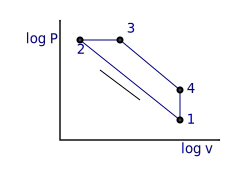
\includegraphics[width=40mm]{fig/idealDieselExample.pdf}
        \caption{Air-standard ideal Diesel cycle in  logarithmic  $P\times  v$  coordinates,  in
            support for the Example~\ref{ex:ideal.Diesel}.}
    \end{figure}

    Now we're in a position to define \emph{exact polytropic process}:

    \begin{definition}[exact polytropic process]\label{def:exact.poly.proc}
        An exact polytropic process is a logical process for which there is a unique  polytropic
        relation $Pv^n = \mbox{const.}$, with a unique, constant exponent $n$, that  holds  true
        for all states in the process path; or an isochoric logical process.
    \end{definition}

    It is worth noting that isochoric processes are equivalent to polytropic processes  with  $n
    \to \pm\infty$ between stated end states. Definition~\ref{def:exact.poly.proc} accounts  for
    the isochoric process non-unique polytropic exponent by explicitly including it as  a  valid
    exact polytropic process.

    \begin{theorem}\label{cor:1}
        Any logical process defined by  a  unique,  constant-polytropic  exponent  relation  and
        non-identical end states---beyond which the defining polytropic relation no longer holds
        true---is an exact polytropic process.
    \end{theorem}

    \begin{proof}
        Such logical process definition statement fulfills the definition criteria for an  exact
        polytropic process, and therefore, is by definition, an exact polytropic process.  Since
        the definition prohibits  the  end  states  to  be  identical,  the  uniqueness  of  the
        polytropic relation is guaranteed, for if end states ``1'' and ``2'' are identical, then
        $P_1v_1^n = P_2v_2^n$ for any exponent $n$ since $P_1 = P_2$ and $v_1 = v_2$; otherwise,
        only the defining $n$ would cause the relation to  hold  true  for  all  states  in  the
        process path.
    \end{proof}



%-----------------------------------------------------------------------------------------------
\section*{Acknowledgments}

    This research received no specific grant from any funding agency in the public, private,  or
    not-for-profit sectors.

%-----------------------------------------------------------------------------------------------

\bibliographystyle{plain}
\bibliography{bibfile}

%-----------------------------------------------------------------------------------------------
\end{multicols*}

%-----------------------------------------------------------------------------------------------
\end{document}
%-----------------------------------------------------------------------------------------------
